\chapter{Экспериментально-исследовательский раздел}

\section{Методология исследования}
Настоящее исследование направлено на сравнительный анализ языковых моделей применительно к задаче декомпозиции сложных вопросов. Основной фокус исследования — оценка качества декомпозиции и изучение практической применимости моделей в условиях ограниченных вычислительных ресурсов. В рамках исследования были проанализированы 30 языковых моделей, рассмотренных в аналитической части работы.

Необходимо отметить, что изначальный план исследования предполагал измерение времени обработки и потребления памяти моделями при выполнении декомпозиции. Однако в ходе работы выяснилось, что большинство рассмотренных в аналитическом разделе языковых моделей требует значительных вычислительных ресурсов, недоступных в рамках данного исследования. По этой причине основной акцент был сделан на экспертной оценке качества декомпозиции.

\subsection{Тестовая выборка}
Для проведения исследования была сформирована тестовая выборка из 10 сложных вопросов, охватывающих различные предметные области. Критериями отбора вопросов служили многокомпонентность (наличие нескольких аспектов, требующих рассмотрения), тематическое разнообразие и структурная сложность. Тестовая выборка представлена в таблице~\ref{tab:test-questions}.

\begin{table}[H]
	\caption{Тестовая выборка сложных вопросов}
	\label{tab:test-questions}
	\begin{tabular}{|p{0.5cm}|p{15.6cm}|}
		\hline
		\textbf{№} & \textbf{Вопрос} \\
		\hline
		1 & Какие факторы повлияли на развитие письменности в древних цивилизациях и как это изменило политическую, экономическую и социальную структуру общества? \\
		\hline
		2 & Как экологические проблемы, связанные с загрязнением океана пластиком, влияют на морских обитателей, прибрежные экосистемы и здоровье человека, и какие существуют технологические и законодательные решения для минимизации этого воздействия? \\
		\hline
		3 & Каково влияние искусственного интеллекта на рынок труда, образование и этические нормы общества, и как следует регулировать его развитие? \\
		\hline
		4 & Какие технологические прорывы в области квантовых вычислений могут изменить подход к криптографии и обработке больших данных в ближайшие десятилетия? \\
		\hline
		5 & Как глобализация повлияла на культурную идентичность малых народов и какие существуют стратегии сохранения языкового разнообразия? \\
		\hline
		6 & Какие медицинские, этические и юридические аспекты необходимо учитывать при внедрении генной инженерии в клиническую практику? \\
		\hline
		7 & Как развитие возобновляемых источников энергии изменяет геополитическую ситуацию и экономику стран-экспортеров нефти? \\
		\hline
		8 & Какие философские концепции лежат в основе современных подходов к искусственному интеллекту и как они влияют на его восприятие обществом? \\
		\hline
		9 & Какие нейробиологические механизмы ответственны за формирование долговременной памяти и как их понимание может помочь в лечении нейродегенеративных заболеваний? \\
		\hline
		10 & Как цифровизация образования влияет на когнитивное развитие студентов и какие риски она несет для традиционной педагогики? \\
		\hline
	\end{tabular}
\end{table}

\section{Оценка качества декомпозиции}
Оценка качества декомпозиции сложных вопросов проводилась экспертным методом. Для этого каждая из 30 исследуемых моделей использовалась для разбиения всех 10 вопросов из тестовой выборки. Полученные результаты анализировались квалифицированным экспертом с опытом в области лингвистики и обработки естественного языка.

С целью обеспечения объективности оценки был разработан комплекс критериев для стандартизации процесса экспертной оценки. Это позволило минимизировать субъективность и получить сопоставимые результаты для разных моделей.

\subsection{Критерии экспертной оценки}
Оценка качества декомпозиции проводилась по трем ключевым критериям:

\textbf{Полнота} (0-5 баллов): оценивает степень охвата всех смысловых аспектов исходного вопроса. Максимальный балл присваивался, если полученный набор подвопросов полностью покрывал информационную потребность исходного вопроса.

\textbf{Атомарность} (0-5 баллов): оценивает степень фокусировки каждого подвопроса на одном смысловом компоненте. Высокий балл присваивался, если подвопросы не содержали несколько разнородных аспектов и не требовали дальнейшей декомпозиции.

\textbf{Корректность} (0-5 баллов): оценивает грамматическую и логическую целостность подвопросов. Критерий учитывал логичность формулировок, отсутствие грамматических ошибок и стилистическую согласованность.

Процесс получения итоговой оценки включал два этапа усреднения. Сначала для каждой модели по каждому из трех критериев вычислялось среднее арифметическое оценок за все 10 тестовых вопросов. Затем полученные три средних значения (по полноте, атомарности и корректности) усреднялись, формируя итоговый показатель качества декомпозиции. Данный подход обеспечил комплексную оценку производительности моделей с учетом всех аспектов качества декомпозиции.

\subsection{Результаты оценки}
На основе анализа результатов декомпозиции 10 тестовых вопросов была составлена сводная таблица экспертных оценок по всем 30 исследуемым моделям (таблица~\ref{tab:expert-results-full}). Модели в таблице расположены в порядке убывания среднего балла.

\begin{table}[H]
	\caption{Сводные результаты экспертной оценки качества декомпозиции сложных вопросов}
	\label{tab:expert-results-full}
	\begin{tabular}{|l|B|B|B|B|}
		\hline
		\textbf{Модель} & \textbf{Полнота} & \textbf{Атомарность} & \textbf{Корректность} & \textbf{Средний балл} \\
		\hline
		DeepSeek-V3-Chat & 4.8 & 4.6 & 4.9 & 4.77 \\
		chatgpt-4o-latest & 4.7 & 4.5 & 4.8 & 4.67 \\
		claude-3-opus-20240229 & 4.4 & 4.5 & 4.7 & 4.53 \\
		o1-mini & 4.5 & 4.2 & 4.6 & 4.43 \\
		RuadaptQwen-32B-Pro\_v1 & 4.3 & 4.1 & 4.2 & 4.20 \\
		T-Tech-T-pro-it-1.0 & 4.2 & 4.1 & 4.3 & 4.20 \\
		yi-lightning & 4.3 & 4.1 & 4.2 & 4.20 \\
		gemini-1.5-pro-002 & 4.3 & 4.0 & 4.2 & 4.17 \\
		SberDevices-GigaChatMax & 4.0 & 4.3 & 4.0 & 4.10 \\
		Qwen2.5-72B-Instruct & 4.2 & 3.8 & 4.0 & 4.00 \\
		ru-Zero-Mistral-Small-24B & 3.9 & 4.0 & 4.1 & 4.00 \\
		Phi-4 & 3.9 & 3.7 & 4.3 & 3.97 \\
		llama-3.1-70b-instruct & 3.9 & 3.6 & 4.1 & 3.87 \\
		vikhr-nemo-12b-instruct-r & 3.8 & 4.0 & 3.8 & 3.87 \\
		mistral-large-2407 & 3.8 & 3.8 & 3.6 & 3.73 \\
		gemma-2-9b-it & 3.6 & 3.5 & 3.8 & 3.63 \\
		command-r-plus & 3.6 & 3.6 & 3.6 & 3.60 \\
		Watari-7b-v1 & 3.3 & 3.2 & 3.2 & 3.23 \\
		gpt-3.5-turbo-0125 & 2.9 & 3.5 & 3.1 & 3.17 \\
		MTSAIR-Cotype-Nano & 3.4 & 2.8 & 3.2 & 3.13 \\
		yandexgpt-4-pro & 3.2 & 3.1 & 3.1 & 3.13 \\
		glm-4-9b-chat & 2.9 & 2.8 & 3.1 & 2.93 \\
		c4ai-command-r-v01 & 2.7 & 2.8 & 2.7 & 2.73 \\
		hermes-2-theta-llama-3-8b & 2.6 & 2.7 & 2.8 & 2.70 \\
		suzume-llama-3-8b-multilingual & 2.7 & 2.6 & 2.8 & 2.70 \\
		saiga\_llama3\_8b\_v6 & 2.5 & 2.6 & 2.7 & 2.60 \\
		paralex-llama-3-8b-sft & 2.5 & 2.4 & 2.6 & 2.50 \\
		aya-23-8b & 2.4 & 2.3 & 2.5 & 2.40 \\
		storm-7b & 2.2 & 2.2 & 2.3 & 2.23 \\
		neural-chat-7b-v3-3 & 2.2 & 2.1 & 2.2 & 2.17 \\
		\hline
	\end{tabular}
\end{table}

\begin{figure}[H]
	\centering
	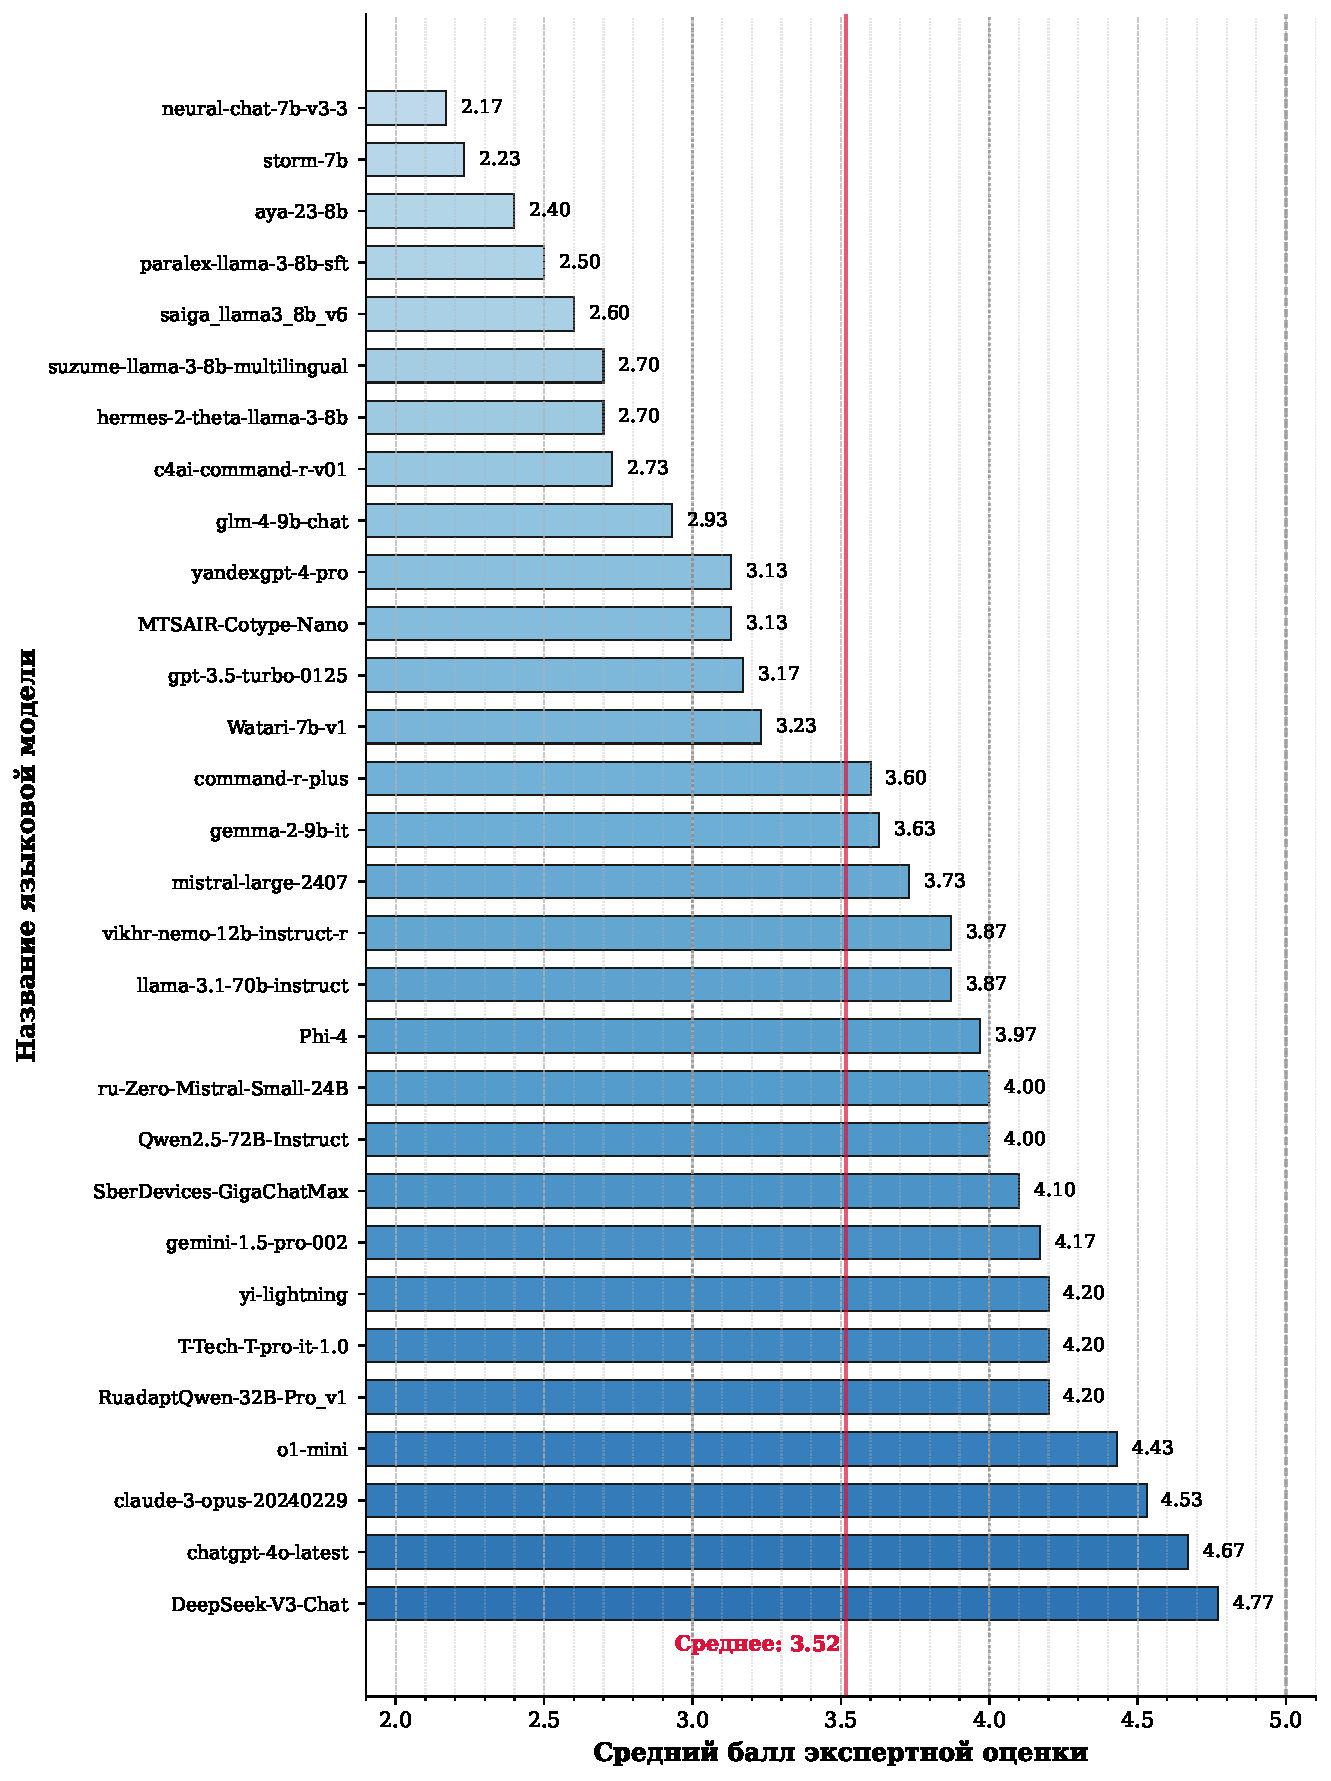
\includegraphics[width=1\textwidth]{images/model_performance_comparison.pdf}
	\caption{Сравнение моделей по интегральному показателю качества}
	\label{fig:quality}
\end{figure}

Проведенное исследование показало, что наилучшие результаты демонстрируют проприетарные модели DeepSeek-V3-Chat, chatgpt-4o-latest и Claude-3-Opus, доступные только через API. Среди локальных моделей высокие результаты показывают T-Tech-T-pro-it-1.0 и RuadaptQwen-32B-Pro\_v1 с показателем 4.20 балла, что подтверждает высокое качество этих открытых моделей.

\section{Практические ограничения}
Несмотря на значительное превосходство проприетарных моделей и крупных локальных моделей в качестве декомпозиции, их практическое применение сталкивается с серьезными ограничениями. Эти ограничения имеют существенное влияние на возможность проведения комплексного исследования всех аспектов работы моделей.

Анализ доступности моделей показал, что значительная часть решений с наивысшими показателями качества доступна исключительно через API, что делает невозможным их локальное развертывание. Такие модели как DeepSeek-V3-Chat, chatgpt-4o-latest, claude-3-opus, o1-mini, gemini-1.5-pro, SberDevices-GigaChatMax и другие могут использоваться только при наличии подключения к соответствующим сервисам и с учетом ограничений, устанавливаемых поставщиками этих сервисов.

Среди моделей, теоретически доступных для локального запуска, также существует значительное расслоение по требованиям к вычислительным ресурсам. Крупные модели, такие как LLaMA-3.1-70b-instruct (39.8 ГБ), Qwen2.5-72B (40.6 ГБ) и mistral-large-2407 (45.3 ГБ), требуют не менее 80-92 ГБ оперативной памяти, что существенно превышает возможности стандартных персональных компьютеров и требует специализированного серверного оборудования. Модели среднего размера, включая RuadaptQwen-32B (18.3 ГБ) и T-Tech-T-pro-it-1.0 (16.4 ГБ), хотя и требуют меньше ресурсов, всё равно выходят за рамки возможностей рядового пользовательского оборудования.

Данное ограничение не позволило провести полноценное исследование времени обработки и потребления памяти для большинства моделей, рассмотренных в аналитическом разделе, так как исследовательская среда имела в распоряжении только 8 ГБ оперативной памяти и не обладала специализированным графическим ускорителем, необходимым для эффективной работы крупных моделей.

Более того, сравнительный анализ компактных моделей (<10 ГБ), которые потенциально могли бы быть запущены в исследовательской среде, представляется малоинформативным по двум причинам. Во-первых, большинство таких моделей демонстрируют схожие характеристики производительности при работе на однотипном оборудовании, что обусловлено схожестью их архитектур и методов оптимизации. Во-вторых, детальное измерение производительности требует специализированных методик профилирования, позволяющих отделить собственно время инференса от операций пред- и постобработки текста, что выходит за рамки настоящего исследования.

Таким образом, основной фокус исследования был смещен в сторону оценки качества декомпозиции, которое может быть надежно измерено для всех моделей независимо от их доступности для локального запуска.

\subsection{Выбор модели для практической реализации}
Учитывая описанные выше ограничения и результаты экспертной оценки, для практической реализации системы декомпозиции вопросов была выбрана локальная квантованная модель T-lite-it-1.0-q4\_k\_m из семейства T Bank. Данный выбор обусловлен следующими факторами:

\begin{itemize}
	\item модель T-Tech-T-pro-it-1.0 из того же семейства продемонстрировала наилучшие результаты среди локальных моделей с оценкой 4.20 балла, что указывает на высокую эффективность архитектуры и обучения моделей этого семейства;
	
	\item несмотря на превосходные результаты, модель T-Tech-T-pro-it-1.0 требует 36 ГБ оперативной памяти, что превышает доступные ресурсы исследовательской среды;
	
	\item компактная модель T-lite-it-1.0-q4\_k\_m из того же семейства сохраняет базовые архитектурные особенности и обучающие данные, имея при этом существенно меньшие требования к ресурсам;
	
	\item размер модели составляет 4.68 ГБ, что позволяет запускать ее на стандартном персональном компьютере с ограниченными ресурсами;
	
	\item требуемый объем оперативной памяти не превышает 6 ГБ, что делает модель доступной для подавляющего большинства современных компьютеров;
	
	\item квантованная архитектура модели обеспечивает приемлемую скорость работы даже без использования графического ускорителя. \cite{t_lite_it_q4}
\end{itemize}


\section{Вывод}
Проприетарные модели, доступные через API, демонстрируют наивысшее качество декомпозиции сложных вопросов с оценками 4.77, 4.67 и 4.53 баллов для DeepSeek-V3-Chat, chatgpt-4o-latest и Claude-3-Opus соответственно. Однако их использование требует постоянного подключения к интернету и зависит от доступности и политики стороннего сервиса.

Среди локальных моделей наилучшие результаты показывает T-Tech-T-pro-it-1.0 с оценкой 4.20 баллов, что подтверждает высокое качество моделей семейства T Bank. Данная модель может считаться эталоном качества для решений, работающих без доступа к сети, однако требует значительных вычислительных ресурсов, недоступных на стандартных персональных компьютерах.

Квантованная модель T-lite-it-1.0-q4\_k\_m представляет собой оптимальный компромисс между качеством декомпозиции и возможностью запуска на потребительском оборудовании. Несмотря на более низкий показатель качества по сравнению с проприетарными решениями, модель обеспечивает приемлемый уровень декомпозиции и может быть успешно использована в практических приложениях.

Таким образом, исследование показало возможность эффективной декомпозиции сложных вопросов с использованием языковых моделей различного масштаба, что открывает перспективы для создания практических приложений, способных работать в условиях ограниченных вычислительных ресурсов.